\documentclass[a4paper]{article}
\usepackage[polish]{babel}
\usepackage{polski}
\usepackage[utf8]{inputenc}
\usepackage[T1]{fontenc}
\usepackage[a4paper,top=3cm,bottom=2cm,left=3cm,right=3cm,marginparwidth=1.75cm]{geometry}
\usepackage{graphicx}
\usepackage{amsmath}
\usepackage{float}
\usepackage{listings}
\graphicspath{{img/}} 

\usepackage[pdftex,
            pdfauthor={Artur Bauer},
            pdftitle={Optymalizacja wielokryterialna},
            pdfsubject={Optymalizacja wielokryterialna},
            pdfkeywords={Optymalizacja wielokryterialna},
            pdfproducer={Latex},
            pdfcreator={pdflatex}]{hyperref}
            
\usepackage[backend=biber,
            style=alphabetic,
            ]{biblatex}
\addbibresource{bibl.bib}
            
\title{Projekt przekładni}
\author{Artur Bauer}
\def \nazwa_przedmiotu{Optymalizacja wielokryterialna}
\title{Problemy wielokryterialnego sterowania optymalnego}

\begin{document}

\begin{titlepage}
\makeatletter

\newcommand{\HRule}{\rule{\linewidth}{0.5mm}} % Defines a new command for the horizontal lines, change thickness here

\center % Center everything on the page
 
%----------------------------------------------------------------------------------------
%	HEADING SECTIONS
%----------------------------------------------------------------------------------------

\textsc{\LARGE Akademia Górniczo Hutnicza}\\[1.5cm] % Name of your university/college
\textsc{\nazwa_przedmiotu}\\[0.5cm] % Major heading such as course name
%\textsc{\large Projekt}\\[0.5cm] % Minor heading such as course title

%----------------------------------------------------------------------------------------
%	TITLE SECTION
%----------------------------------------------------------------------------------------

\HRule \\[0.4cm]
{ \huge \bfseries \@title} \\[1.4cm] % Title of your document
\HRule \\[1.5cm]
 
%----------------------------------------------------------------------------------------
%	AUTHOR SECTION
%----------------------------------------------------------------------------------------

\begin{minipage}{0.4\textwidth}
\begin{flushleft} \large
\emph{Autor:}\\
Artur \textsc{Bauer} % Your name
\end{flushleft}
\end{minipage}
~
\begin{minipage}{0.4\textwidth}
\begin{flushright} \large
\emph{Prowadzący:} \\
prof dr hab. inż. \\Andrzej \textsc{Skulimowski} % Supervisor's Name
\end{flushright}
\end{minipage}\\[2cm]

%----------------------------------------------------------------------------------------
%	DATE SECTION
%----------------------------------------------------------------------------------------

{\large \today}\\[1cm] % Date, change the \today to a set date if you want to be precise

%----------------------------------------------------------------------------------------
%	LOGO SECTION
%----------------------------------------------------------------------------------------


\includegraphics[width=0.4\textwidth]{agh_logo.pdf}\\[1cm] % Include a department/university logo - this will require the graphicx package
 
%----------------------------------------------------------------------------------------

\vfill % Fill the rest of the page with whitespace
\end{titlepage}

\section{Cel ćwiczenia}

% WF = [1.00745726261696e-07	3.24041823661910e-06]
% Optymalizacja wielokryterialna 
% Problem wielokryterialnego sterowania optymalnego (multicriteria optimal control) 

Celem ćwiczenia jest zapoznanie się z problemem wielokryterialnego sterowania optymalnego i przedstawienie własnego toku rozumowania przy rozwiązywaniu tego zagadnienia.  

\section{Definicja problemu}

Dla multi-kryterialnego problemu znajdowania optymalnego sterowania: 
$$ \frac{d}{dx} x(t) = A(t) x(t) + B(t) u(t)$$
$$ x(t_0) := x_0 $$
$$ J_1(x,u,T) = \int^T_0 g_1(x(t), u(t), t) dt, \cdots, J_N(x,u,T) = \int^T_0 g_N(x(t), u(t), t) dt$$
$$ J_1(T) = J_1(x,u,T) $$
$$ ( J_1(T), \cdots, J_N(T) ) \rightarrow min $$
gdzie: 
$ u(t)\in R^k, 0 \leq u_j(t) \leq u_{aj}(t), 1\leq j \leq k $
oraz 
$ A(t), B(t), u_{aj}(t), g_i(x,u,t)$
są ciągłe dla danego odcinka.

\noindent
Znajdź sterowanie $u_{opt}$  i odpowiadającą mu trajektorię $x_{opt}$, która jest niezdominowana dla $t=T$. 

\noindent
Dodatkowymi założeniami są:  
\begin{itemize}
    \item $J(u_{opt}\mid_{[\tau, T]}, x_{opt}\mid_{[\tau, T]})$  jest niezdominowane dla wszystkich $\tau \in [t_1, T]$ i $t1$ jest najmniejsze w tym zbiorze 
\end{itemize}

\section{Rozwiązanie}
Dla zmienionego na konsultacjach przykładu 1 z instrukcji ćw.4, czyli: 

$$ \frac{d}{dx} x(t) = A x(t) + B u(t)$$
$$ J_1(x,u,T) = - \int^T_0 x_1(t) dt, J_2(x,u,T) = \int^T_0 u(t) dt$$
$$ ( J_1(T), \cdots, J_2(T) ) \rightarrow min $$
gdzie: 
\begin{itemize}
    \item $t_0 = 0$
    \item $x_0 = \begin{bmatrix} 1 \\ 0 \end{bmatrix} $
    \item $A = \begin{bmatrix} 1 & 1 \\ 1 & 0 \end{bmatrix} $
    \item $B = \begin{bmatrix} 0 \\ 1 \end{bmatrix} $
    \item $u(t) \in [0, 1] $
\end{itemize}
Szukamy sterowania 
$u_{opt} = 
    \begin{bmatrix}
        u_{opt1}
    \end{bmatrix}
$
oraz odpowiadającej mu trajektorii systemu 
$
    x_{opt} = 
    \begin{bmatrix}
        x_{opt1} \\
        x_{opt2}
    \end{bmatrix}
$
, która jest niezdominowana dla $t=T$ i taka, że: 
\begin{itemize}
    \item $J(u_{opt}\mid_{[\tau, T]})$ jest niezdominowane dla wszystkich $\tau \in [t_1, T]$ oraz $t_1$ jest największe w tym zbiorze. 
\end{itemize}

\subsection{Kroki rozwiązania}
% Z uwagi na ograniczenia sterowania postanowiano przybliżyć je funkcją $u(t)$
\begin{enumerate}
    \item  Obliczenie $J_1$ oraz $J_2$
    \item Znalezienie zbioru rozwiązań niezdominowanych dla $(J_1, J_2)$ w chwili $t=T$
    \item Znalezienie zbioru rozwiązań niezdominowanych dla $(J_1, J_2)$ w chwili $t_1 < T$ oraz porównanie parametrów sterowania 
    \item Powtórzenie kroku 3. aż w zbiorze zostanie tylko jeden parametr sterowania dla czasu $t_1$
    \item  Znalezienie optymalnej trajektorii $x(t)$ dla optymalnej wartości $u(t)$
\end{enumerate}

    
 

\subsubsection{Obliczenie J1 oraz J2}
\label{step:1}
Obliczono $J_1$ oraz $J_2$ dla czasu $T$, co dało następujące wyniki:
\begin{itemize}
    \item $J_1 = - x^2 * 0.5 * T $
    \item $J_2 = - u^2 * 0.5 * T $
\end{itemize}
 
\subsubsection{Znalezienie zbioru rozwiązań niezdominowanych dla $(J_1, J_2)$}
\label{step:2}

Zgodnie z poleceniem znajdujemy taką wartość $u(t)$, dla której $(J_1, J_2) \rightarrow min$, dla $u(t) \in  [0,1]$.
\\
W celu uproszczenia obliczeń jako funkcję $u(t)$ przyjęto $u(t) = 0.5*sign(f*t^ + g*t + h)+0.5$.
\\
Znalezienie optymalnych wartości $(J_1, J_2) \rightarrow min$ zrealizowano przy pomocy funkcji \texttt{paretosearch} pakietu \textit{Matlab}.
\\
Znaleziony zbiór rozwiązań paretooptymalnych (front pareto) przedstawiono na Rys.~\ref{fig:pareto_front}. 
\begin{figure}[H]
    \centering
    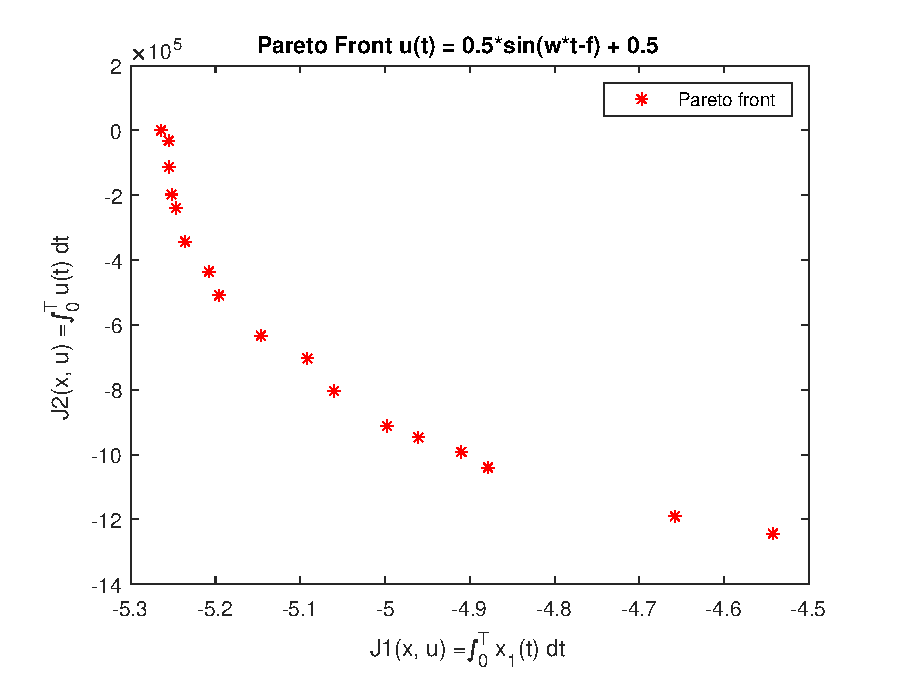
\includegraphics{pareto_front.eps}
    \caption{Front Pareto}
    \label{fig:pareto_front}
\end{figure}

\subsubsection{Znalezienie zbioru rozwiązań niezdominowanych dla $(J_1, J_2)$ w chwili $t_1 < T$ oraz porównanie parametrów sterowania}
\label{step:3}

W celu znalezienia rozwiązania niezdominowanego od zdecydowano się na zmniejszanie maksymalnej wartości $T$.
\\
Dla każdego tak zdefiniowanego momentu $t_1$ wyznaczano front pareto korzystajac z metody opisanej w sekcji~\ref{step:2}.
\\
Następnie porównano zbiór rozwiązań ze zbiorem rozwiązań z poprzedniej iteracji $T \geq t > t_1$ i wykluczono rozwiązania niepowtarzające się.
\\ Krok opisany w sekcji~\ref{step:3} powtarzano aż w zbiorze rozwiązań zostało jedno rozwiązanie. 

\subsubsection{Znalezienie optymalnej trajektorii x odpowiadającej optymalnej wartości u}
\label{step:4}

Dla znalezionej optymalnej wartości $u(t)$ obliczamy optymalną trajektorię korzystając z funkcji \textit{Matlaba} \texttt{ode45()} do rozwiązywania równań różniczkowych. 
\\
Optymalne parametry znalezione przez \textit{Matlab} to 
\begin{itemize}
    \item $f = -2.5 $
    \item $g = 2.5 $
    \item $h = 7.5$,
\end{itemize}
dla funkcji sterowania: $u(t) = 0.5*sign(f*t^2 + g*t + h)+0.5$.
\\Optymalna trajektoria ruchu dla tej funkcji została przedstawiona na Rys.~\ref{fig:trajectory}.
\begin{figure}[H]
    \centering
    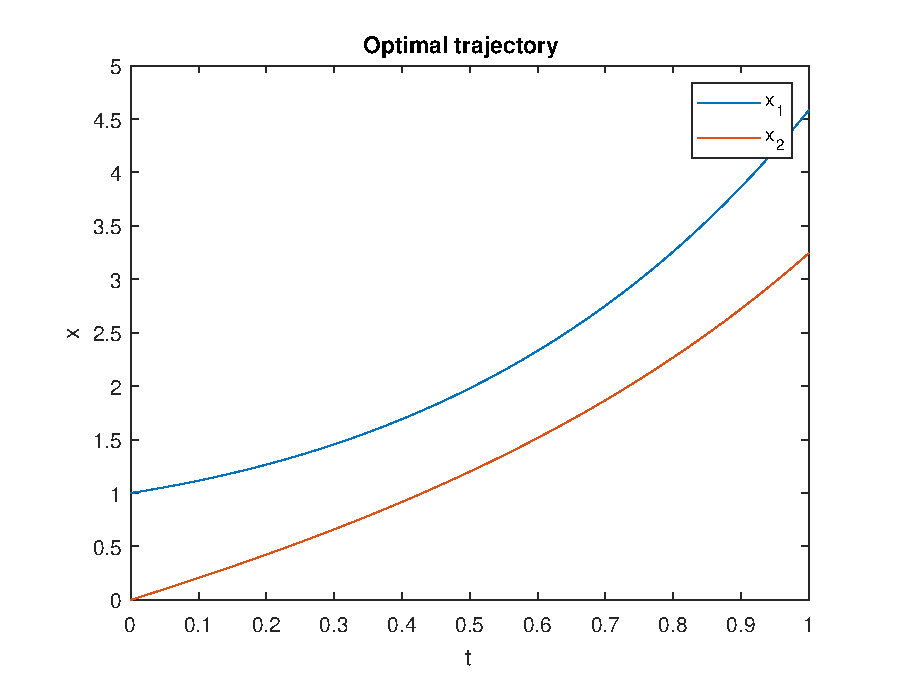
\includegraphics{path.eps}
    \caption{Optymalna trajektoria}
    \label{fig:trajectory}
\end{figure}

\section{Wnioski}
Z uwagi na mało optymalne sterowanie sygnałem sinusoidanlym zdecydowano się na zastosowanie sygnału typu \textit{bang-bang}.
Sterowanie to posiadało maksymalnie 2 przejścia między sygnałami. 
Zdecydowano się na wyciągnięcie znaku wielomianu 2 stopnia i przesunięciu go w osi 0Y.
Konieczna była optymalizacja 3 parametrowa zamiast początkowo przewidzianej 2 parametrowej. 
Całkę obliczono sumując czas, w którym sterowanie miało wartość 1. 


Zrezygnowano z obliczeń metodą \texttt{gamultiobj} na rzecz metody \texttt{paretosearch} co znacząco zwiększyło czas obliczeń, ale pozwoliło na uzyskanie dokładniejszych wyników.

Alternatywną metodą obliczenia sterowania optymalnego byłoby wykorzystanie mnożnika Lagrange analogicznie jak w publikacji \cite{kaya2004computations}.
Z uwagi na inne zobowiązania nie byłem w stanie jednak wykonać implementacji wyżej wymienionego rozwiązania. 


\newpage
\section{Listingi}
\lstinputlisting[caption=Klasa Undmoinated, language=Matlab]{matlab/Nondominated.m}
\lstinputlisting[caption=Skrypt uruchamiający, language=Matlab]{matlab/nonDomTst.m}

\newpage
\printbibliography
\end{document}
